\documentclass{beamer}
% \documentclass[handout,xcolor=pdftex,dvipsnames,table]{beamer}

\mode<presentation>
{
  \usetheme{Warsaw}
  \usecolortheme{whale}
  % or ...

  \setbeamercovered{transparent}
  % or whatever (possibly just delete it)
  \setbeamertemplate{navigation symbols}{}
}

\setbeamertemplate{itemize items}[ball]
\setbeamertemplate{itemize subitem}[triangle]
\setbeamertemplate{itemize subsubitem}[circle]
\setbeamercovered{transparent}

\usepackage{palatino} 
\usepackage{listings} % Gives syntax highlighting for python code. 
\usepackage{color} % Used for syntax highlighting. 
\usepackage{textcomp} % Used for syntax highlighting. 

% This gives syntax highlighting in the python environment 
\definecolor{gray}{gray}{0.5} 
\definecolor{key}{rgb}{0,0.5,0} 
\lstset{
language=python,
basicstyle=\ttfamily\tiny, 
otherkeywords={1, 2, 3, 4, 5, 6, 7, 8 ,9 , 0, -, =, +, [, ], (, ), \{, \}, :, *, !}, 
keywordstyle=\color{blue}, 
stringstyle=\color{red},
showstringspaces=false,
alsoletter={1234567890},
otherkeywords={\ , \}, \{},
keywordstyle=\color{blue},
emph={access,and,break,class,continue,def,del,elif ,else,%
except,exec,finally,for,from,global,if,import,in,is,%
lambda,not,or,pass,print,raise,return,try,while},
emphstyle=\color{black}\bfseries,
emph={[2]True, False, None, self},
emphstyle=[2]\color{green},
emph={[3]from, import, as},
emphstyle=[3]\color{blue},
upquote=true,
morecomment=[s]{"""}{"""},
commentstyle=\color{gray}\slshape,
emph={[4]1, 2, 3, 4, 5, 6, 7, 8, 9, 0},
emphstyle=[4]\color{blue},
literate=*{:}{{\textcolor{blue}:}}{1}%
{=}{{\textcolor{blue}=}}{1}%
{-}{{\textcolor{blue}-}}{1}%
{+}{{\textcolor{blue}+}}{1}%
{*}{{\textcolor{blue}*}}{1}%
{!}{{\textcolor{blue}!}}{1}%
{(}{{\textcolor{blue}(}}{1}%
{)}{{\textcolor{blue})}}{1}%
{[}{{\textcolor{blue}[}}{1}%
{]}{{\textcolor{blue}]}}{1}%
{<}{{\textcolor{blue}<}}{1}%
{>}{{\textcolor{blue}>}}{1},%
numbers=none,
}

\newcommand{\putat}[3]{\begin{picture}(0,0)(0,0)\put(#1,#2){#3}\end{picture}}

\title[]{Python Workshop\\
Numpy Arrays}

\author[Langevin] % (optional, use only with lots of authors)
{C.D.~Langevin}
\institute[USGS] % (optional, but mostly needed)
{
  U.S. Geological Survey\\
  Reston, Virginia, USA
  }

\titlegraphic{
\includegraphics[scale=0.5]{figures/c_USGSid1.pdf}}

\date[UQ12] % (optional, should be abbreviation of conference name)
{USGS National Groundwater Workshop, August 2012}

\subject{Python}


\begin{document}

\begin{frame}
  \titlepage
\end{frame}

%put this pdf image on all following slides
\logo{\vspace{-0.3cm} 
\includegraphics[width=1.5cm]{figures/c_USGSid1.pdf}\hspace*{11.10cm}}  

%\begin{frame}{Outline}
%\tableofcontents
%\end{frame}

%\section{Introduction}
\begin{frame}[fragile]
\frametitle{What is Numpy}
\begin{itemize}
  \item Numpy is the main package for scientific computing using Python
  \item Provides an array object of type ndarray
  \item Many functions and methods available for fast array operations
\end{itemize}
\end{frame}

\begin{frame}[fragile]
\frametitle{Numpy Version}
\begin{itemize}
  \item Numpy can be obtained at \url{http://docs.scipy.org/doc/}
  \item Current version is 1.6.
  \item To determine the installed version
\end{itemize}
  \begin{lstlisting}
In [10]: import numpy

In [11]: print numpy.__version__
1.6.1
  \end{lstlisting}
\end{frame}


\begin{frame}[fragile]
\frametitle{Data Types (dtype)}
\begin{table}
\tiny
\begin{tabular}{l l}
  bool        & Boolean (True or False) stored as a byte                                         \\
  int         & Platform integer (normally either int32 or int64)                                \\
  int8        & Byte (-128 to 127)                                                               \\
  int16       & Integer (-32768 to 32767)                                                        \\
  int32       & Integer (-2147483648 to 2147483647)                                              \\
  int64       & Integer (9223372036854775808 to 9223372036854775807)                             \\
  uint8       & Unsigned integer (0 to 255)                                                      \\
  uint16      & Unsigned integer (0 to 65535)                                                    \\
  uint32      & Unsigned integer (0 to 4294967295)                                               \\
  uint64      & Unsigned integer (0 to 18446744073709551615)                                     \\
  float       & Shorthand for float64.                                                           \\
  float16     & Half precision float: sign bit, 5 bits exponent, 10 bits mantissa                \\
  float32     & Single precision float: sign bit, 8 bits exponent, 23 bits mantissa              \\
  float64     & Double precision float: sign bit, 11 bits exponent, 52 bits mantissa             \\
  complex     & Shorthand for complex128.                                                        \\
  complex64   & Complex number, represented by two 32-bit floats (real and imaginary components) \\
  complex128  & Complex number, represented by two 64-bit floats (real and imaginary components) \\ 
\end{tabular}
\end{table}
\url{http://docs.scipy.org/doc/numpy-1.6.0/user/basics.types.html}
\end{frame}

\section{Creating Arrays}
\begin{frame}[fragile]
\frametitle{Creating an Array}
\begin{itemize}
  \item{Using the built-in \emph{array} function}
  \begin{lstlisting}
In [18]: import numpy

In [19]: a1d = numpy.array([0, 1, 2, 3, 4])

In [20]: a1d
Out[20]: array([0, 1, 2, 3, 4])

In [21]: a2d = numpy.array([ [1, 1, 1, 1], [2, 2, 2, 2] ])

In [22]: a2d
Out[22]:
array([[1, 1, 1, 1],
       [2, 2, 2, 2]])
  \end{lstlisting}
  \item Using the built-in \emph{arange} function
  \begin{lstlisting}
In [25]: a = numpy.arange(10)

In [26]: a
Out[26]: array([0, 1, 2, 3, 4, 5, 6, 7, 8, 9])

In [27]: a = numpy.arange(0, 100, 10)

In [28]: a
Out[28]: array([ 0, 10, 20, 30, 40, 50, 60, 70, 80, 90])
  \end{lstlisting}
\end{itemize}
\end{frame}


\begin{frame}[fragile]
\frametitle{Creating an Array}
\begin{itemize}
  \item{Using the built-in \emph{empty} function}
  \begin{lstlisting}
In [27]: a = empty( (2,2) )

In [28]: a
Out[28]:
array([[  2.16777011e-313,   1.78514665e-296],
       [  2.28748514e-296,   2.43212233e-296]])
  \end{lstlisting}
  \item Using the built-in \emph{zeros} function
  \begin{lstlisting}
In [29]: a = zeros( (2,2) )

In [30]: a
Out[30]:
array([[ 0.,  0.],
       [ 0.,  0.]])
  \end{lstlisting}
  \item Using the built-in \emph{ones} function
  \begin{lstlisting}
In [33]: a = ones( (2,2), dtype=int)

In [34]: a
Out[34]:
array([[1, 1],
       [1, 1]])
  \end{lstlisting}
\end{itemize}
\end{frame}



\begin{frame}[fragile]
\frametitle{Creating an Array}
\begin{itemize}
  \item{Using the built-in linspace function}
  \begin{lstlisting}
In [29]: a = numpy.linspace(0, 1, 7)

In [30]: a
Out[30]:
array([ 0.        ,  0.16666667,  0.33333333,  0.5       ,  0.66666667,
        0.83333333,  1.        ])
  \end{lstlisting}

  \item{Universal functions operate elementwise on an array and produce a new array as a result}
  \begin{lstlisting}
In [16]: import numpy

In [17]: x = numpy.linspace(0, 2 * numpy.pi, 20)

In [18]: y = numpy.sin(x)

In [19]: plot(x, y)
Out[19]: [<matplotlib.lines.Line2D object at 0x04A7B8B0>]

In [20]: show()
  \end{lstlisting}

\end{itemize}
\end{frame}

\begin{frame}[fragile]
\frametitle{Loading an Array from a File}
  \centering
    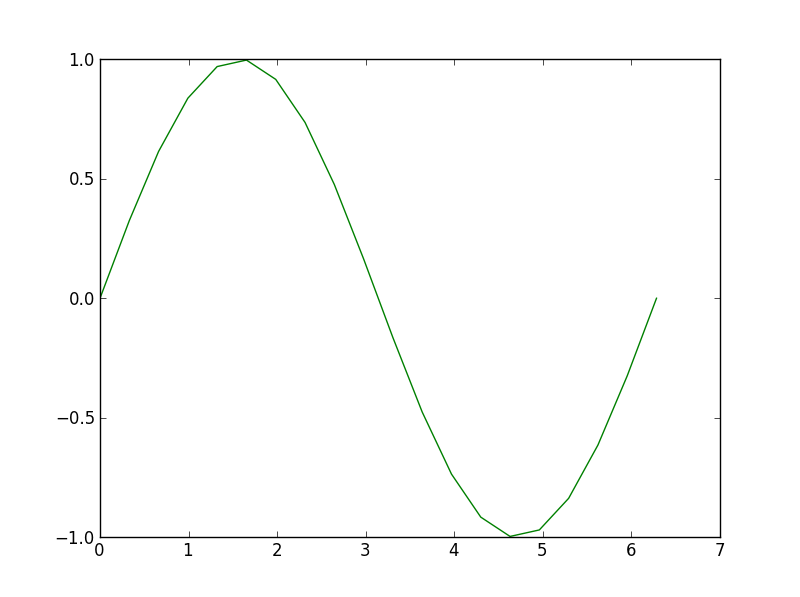
\includegraphics[width=.7\textwidth]{figures/sinx.png} 
\end{frame}

\begin{frame}[fragile]
\frametitle{Loading an Array from a File}
\begin{itemize}
\item{If we have the following table stored in an ascii text file}
\begin{tabular}{l l l l}
  1 & 3 & 6 & 9 \\
  12 & 15 & 18 & 21 \\
  23 & 26 & 29 & 31 \\
  77 & 78 & 79 & 2 \\
\end{tabular}
\item{The table can be loaded into a numpy array using the numpy loadtxt function}
\begin{lstlisting}
In [28]: a = numpy.loadtxt('data\\4by4array.txt')

In [29]: a
Out[29]:
array([[  1.,   3.,   6.,   9.],
       [ 12.,  15.,  18.,  21.],
       [ 23.,  26.,  29.,  31.],
       [ 77.,  78.,  79.,   2.]])
\end{lstlisting}
\end{itemize}
\end{frame}

\section{Indexing, Slicing, Reshaping}
\begin{frame}[fragile]
\frametitle{Array Indexing}
  \begin{itemize}
    \item{Indexing is the term used to access elements in an array}
    \item{One of the biggest gotchas is that numpy arrays are zero-based, which means that the first element of the array is in position zero}
    \begin{lstlisting}
In [9]: a = numpy.arange(1,10)

In [10]: a
Out[10]: array([1, 2, 3, 4, 5, 6, 7, 8, 9])

In [11]: a[0]
Out[11]: 1
    \end{lstlisting}
    \item{Negative indices can be used to go backward through an array}
    \begin{lstlisting}
In [12]: a[-1]
Out[12]: 9

In [13]: a[-2]
Out[13]: 8
    \end{lstlisting}
  \end{itemize}
\end{frame}


\begin{frame}[fragile]
\frametitle{Array Slicing}
  \begin{itemize}
    \item{Slicing is the process of extracting multiple array elements}
    \item{Slicing returns an array}
    \begin{lstlisting}
In [14]: a
Out[14]: array([1, 2, 3, 4, 5, 6, 7, 8, 9])

In [15]: a[2:5]
Out[15]: array([3, 4, 5])

In [16]: a[:2]
Out[16]: array([1, 2])

In [17]: a[5:]
Out[17]: array([6, 7, 8, 9])
    \end{lstlisting}
    \item{Format for slicing is \emph{array[start:end:increment]}}
    \item{Note that the slice is up to the end but not including it}
  \end{itemize}
\end{frame}


\begin{frame}[fragile]
\frametitle{Array Slicing Examples}
  \begin{itemize}
    \item{Every third value}
    \begin{lstlisting}
In [42]: arange(99)[::3]
Out[42]:
array([ 0,  3,  6,  9, 12, 15, 18, 21, 24, 27, 30, 33, 36, 39, 42, 45, 48,
       51, 54, 57, 60, 63, 66, 69, 72, 75, 78, 81, 84, 87, 90, 93, 96])
    \end{lstlisting}
    \item{Every third value up to, but not including position 50}
    \begin{lstlisting}
In [43]: arange(99)[:50:3]
Out[43]: array([ 0,  3,  6,  9, 12, 15, 18, 21, 24, 27, 30, 33, 36, 39, 42, 45,
48])
    \end{lstlisting}
  \end{itemize}
\end{frame}


\begin{frame}[fragile]
\frametitle{Views Verus Copies}
  \begin{itemize}
    \item{Slicing produces a view of an array, not a copy!}
    \begin{lstlisting}
In [44]: a = arange(10)

In [45]: b = a[7:]

In [46]: a
Out[46]: array([0, 1, 2, 3, 4, 5, 6, 7, 8, 9])

In [47]: b
Out[47]: array([7, 8, 9])

In [48]: a[-1] = 1000

In [49]: a
Out[49]: array([   0,    1,    2,    3,    4,    5,    6,    7,    8, 1000])

In [50]: b
Out[50]: array([   7,    8, 1000])

In [51]: a is b
Out[51]: False

In [52]: a is b.base
Out[52]: True
    \end{lstlisting}
  \end{itemize}
\end{frame}


\begin{frame}[fragile]
\frametitle{Shape Manipulation}
  \begin{itemize}
    \item{The shape of an array is stored with the array and can be accessed by a.shape}
    \begin{lstlisting}
In [61]: a = numpy.empty( (2, 3, 4) )

In [62]: a.shape
Out[62]: (2, 3, 4)
    \end{lstlisting}
    \item{The \emph{reshape} method can be used to reshape an array provided a valid shape is given}
    \begin{lstlisting}
In [58]: a = arange(81).reshape(9,9)

In [59]: a
Out[59]:
array([[ 0,  1,  2,  3,  4,  5,  6,  7,  8],
       [ 9, 10, 11, 12, 13, 14, 15, 16, 17],
       [18, 19, 20, 21, 22, 23, 24, 25, 26],
       [27, 28, 29, 30, 31, 32, 33, 34, 35],
       [36, 37, 38, 39, 40, 41, 42, 43, 44],
       [45, 46, 47, 48, 49, 50, 51, 52, 53],
       [54, 55, 56, 57, 58, 59, 60, 61, 62],
       [63, 64, 65, 66, 67, 68, 69, 70, 71],
       [72, 73, 74, 75, 76, 77, 78, 79, 80]])
    \end{lstlisting}
  \end{itemize}
\end{frame}

\section{Helpful Hints}
\begin{frame}[fragile]
\frametitle{Helpful Methods and Functions}
  \begin{itemize}
    \item{min, max, mean, sum}
    \begin{lstlisting}
In [76]: import numpy.random

In [77]: a = numpy.random.random( (50) )

In [78]: a
Out[78]:
array([ 0.55414299,  0.3271058 ,  0.31632925,  0.47979442,  0.25520635,
        0.80985775,  0.81492243,  0.85632766,  0.09273485,  0.56799651,
        0.04924593,  0.51993142,  0.60822579,  0.24912596,  0.06104689,
        0.29200259,  0.42240031,  0.4868186 ,  0.35386243,  0.70139757,
        0.07047982,  0.40676585,  0.1478561 ,  0.42732459,  0.11536969,
        0.50936407,  0.01519514,  0.484014  ,  0.81256495,  0.61565382,
        0.31964842,  0.41620434,  0.13149336,  0.60968828,  0.93935494,
        0.7523049 ,  0.56316456,  0.51333611,  0.03416447,  0.70446818,
        0.57875077,  0.78433295,  0.14120873,  0.99182476,  0.10675879,
        0.99531427,  0.66518705,  0.29422553,  0.26866666,  0.3063704 ])

In [79]: a.min()
Out[79]: 0.015195139324459928

In [80]: a.max()
Out[80]: 0.99531427387945004

In [81]: a.mean()
Out[81]: 0.45079062017573351

In [82]: a.sum()
Out[82]: 22.539531008786675
    \end{lstlisting}
  \end{itemize}
\end{frame}


\begin{frame}[fragile]
\frametitle{Helpful Methods and Functions}
  \begin{itemize}
    \item{\emph{where} can be used to find the indices where some condition is true}
    \begin{lstlisting}
In [109]: ibound
Out[109]:
array([[1, 1, 1, 1, 1, 1, 1, 0, 0, 0],
       [1, 1, 1, 1, 1, 1, 1, 0, 0, 0],
       [1, 1, 1, 1, 1, 1, 1, 0, 0, 0],
       [1, 1, 1, 1, 1, 1, 1, 1, 1, 1],
       [1, 1, 1, 1, 1, 1, 1, 1, 1, 1],
       [1, 1, 1, 1, 1, 1, 1, 1, 1, 1],
       [1, 1, 1, 1, 1, 1, 1, 1, 1, 1],
       [1, 1, 1, 1, 1, 1, 1, 1, 1, 1],
       [1, 1, 1, 1, 1, 1, 1, 1, 1, 1],
       [1, 1, 1, 1, 1, 1, 1, 1, 1, 1]])

In [110]: idx_active = numpy.where(ibound > 0)

In [111]: idx_active
Out[111]:
(array([0, 0, 0, 0, 0, 0, 0, 1, 1, 1, 1, 1, 1, 1, 2, 2, 2, 2, 2, 2, 2, 3, 3,
       3, 3, 3, 3, 3, 3, 3, 3, 4, 4, 4, 4, 4, 4, 4, 4, 4, 4, 5, 5, 5, 5, 5,
       5, 5, 5, 5, 5, 6, 6, 6, 6, 6, 6, 6, 6, 6, 6, 7, 7, 7, 7, 7, 7, 7, 7,
       7, 7, 8, 8, 8, 8, 8, 8, 8, 8, 8, 8, 9, 9, 9, 9, 9, 9, 9, 9, 9, 9]),
 array([0, 1, 2, 3, 4, 5, 6, 0, 1, 2, 3, 4, 5, 6, 0, 1, 2, 3, 4, 5, 6, 0, 1,
       2, 3, 4, 5, 6, 7, 8, 9, 0, 1, 2, 3, 4, 5, 6, 7, 8, 9, 0, 1, 2, 3, 4,
       5, 6, 7, 8, 9, 0, 1, 2, 3, 4, 5, 6, 7, 8, 9, 0, 1, 2, 3, 4, 5, 6, 7,
       8, 9, 0, 1, 2, 3, 4, 5, 6, 7, 8, 9, 0, 1, 2, 3, 4, 5, 6, 7, 8, 9]))
    \end{lstlisting}
  \end{itemize}
\end{frame}


\begin{frame}[fragile]
\frametitle{Helpful Methods and Functions}
  \begin{itemize}
    \item{The indices can be used to access array elements}
    \begin{lstlisting}
In [136]: head = numpy.random.random( (10, 10) ) * 100.

In [137]: head
Out[137]:
array([[  4.26240427e+01,   1.57995831e+01,   2.99365654e+01,
          6.33632715e+01,   3.94482417e+01,   1.49308627e+01,
          8.60771838e+01,   6.28894526e+01,   2.12602996e+01,
          1.89363873e+01],
...
       [  4.42445323e+01,   9.66760310e+01,   2.61880066e+01,
          5.00637180e+01,   7.34959659e+01,   3.57624988e+01,
          2.09579933e+00,   2.37504240e+01,   7.04080247e+01,
          8.49936631e+01]])

In [138]: print head.min(), head.max(), head.sum()
0.0629813630584 99.6093486525 4859.4605162

In [139]: print head[idx_active].min(), head[idx_active].max(), head[idx_active]
.sum()
0.0629813630584 99.6093486525 4339.2850813
    \end{lstlisting}
  \end{itemize}
\end{frame}

\begin{frame}[fragile]
\frametitle{Helpful Methods and Functions}
  \begin{itemize}
    \item{The indices can be used to assign values to array elements}
    \begin{lstlisting}
In [140]: idx_inactive = where(ibound == 0)

In [141]: head[idx_inactive] = -999.

In [142]: head
Out[142]:
array([[  4.26240427e+01,   1.57995831e+01,   2.99365654e+01,
          6.33632715e+01,   3.94482417e+01,   1.49308627e+01,
          8.60771838e+01,  -9.99000000e+02,  -9.99000000e+02,
         -9.99000000e+02],
...
       [  4.42445323e+01,   9.66760310e+01,   2.61880066e+01,
          5.00637180e+01,   7.34959659e+01,   3.57624988e+01,
          2.09579933e+00,   2.37504240e+01,   7.04080247e+01,
          8.49936631e+01]])
    \end{lstlisting}
  \end{itemize}
\end{frame}

\begin{frame}[fragile]
\frametitle{Helpful Methods and Functions}
  \begin{itemize}
    \item{\emph{where} can also be used to build a new array}
    \item{\emph{where(condition, [x, y])}: x is inserted where the condition is true and y where the condition is false}
    \begin{lstlisting}
In [143]: where( ibound == 0, -999, head)
Out[143]:
array([[  4.26240427e+01,   1.57995831e+01,   2.99365654e+01,
          6.33632715e+01,   3.94482417e+01,   1.49308627e+01,
          8.60771838e+01,  -9.99000000e+02,  -9.99000000e+02,
         -9.99000000e+02],
...
       [  4.42445323e+01,   9.66760310e+01,   2.61880066e+01,
          5.00637180e+01,   7.34959659e+01,   3.57624988e+01,
          2.09579933e+00,   2.37504240e+01,   7.04080247e+01,
          8.49936631e+01]])
    \end{lstlisting}
  \end{itemize}
\end{frame}


\begin{frame}[fragile]
\frametitle{Summary}
\begin{itemize}
  \item{Numpy provides a great way to work with arrays.  It provides the foundation for working with groundwater models}
  \item{Don't forget the zero-based indexing!}
  \item{The number of functions and methods can be overwhelming.  The best way to become proficient is to start using it.  Lots of information available on the internet.}
\end{itemize}
\end{frame}


\begin{frame}{Putting it all together: Theis Example}
  \small{\texttt{theis.py}}
  \begin{figure}[ht]
  \centering
        \lstset{numbers=left}
        \lstinputlisting[language=python, firstnumber=1]{python/theis.py}
   \end{figure}
   \putat{200}{10}{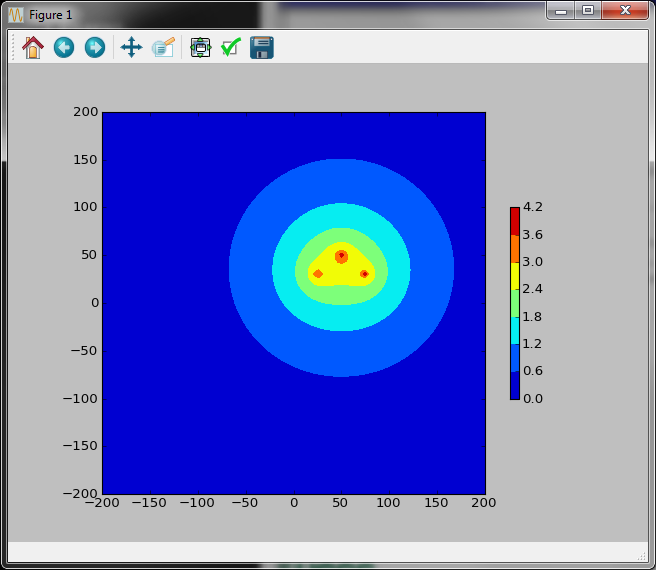
\includegraphics[width=4.0cm]{figures/theis.png} }
\end{frame}



\end{document}